\chapter{Introduction}

% Trends of the electronic field is size reduction
La miniaturization des circuits électroniques se poursuit malgré des barrières technologiques de plus en plus élevées.
La diminution de taille des circuits intégrés permet une réduction des coûts grâce à l'augmentation des volumes de production.
La réduction de poids des modules électroniques pour l'automobile ou l'aéronautique permet des réductions de carburant, de coût, et moins d'impact sur l'environnement.
A taille constante, des circuit intégrés plus denses peuvent embarquer plus de fonctionnalités et ont des performances plus élevées.

% How is size reduced
La réduction de taille des circuits intégrés est possible en utilisant des technologies silicium plus fines.
Une technologie silicium définie les dimensions et les formes d'un ensemble de briques de conception électronique, formant une librairie de composants, ainsi que tous les procédés nécessaires à la fabrication du circuit intégré.
La plupart du temps, ces librairies de composant sont constituées de différents types de transistors, diode, résistances et capacitances.
La taille d'une technologie est définie par la plus petite dimension possible pour une grille de transistor, aussi appellée \textlambda.
La valeur de \textlambda est essentielle et conditionne fortement la taille du circuit final, sa consommation et ses performances.
Jusqu'à présent, la loi de Moore a prédit avec succès que \textlambda serait réduit d'un facteur deux tous les dix-huit mois.
Le domaine automobile se conforme à cette tendance, en utilisant récemment des noeuds technologiques à 16nm (Fig. \ref{fig:nxp-techno-increase}) \cite{evolution_technologies} normalement utilisés dans des applications moins sévères.

\begin{figure}[!h]
  \centering
  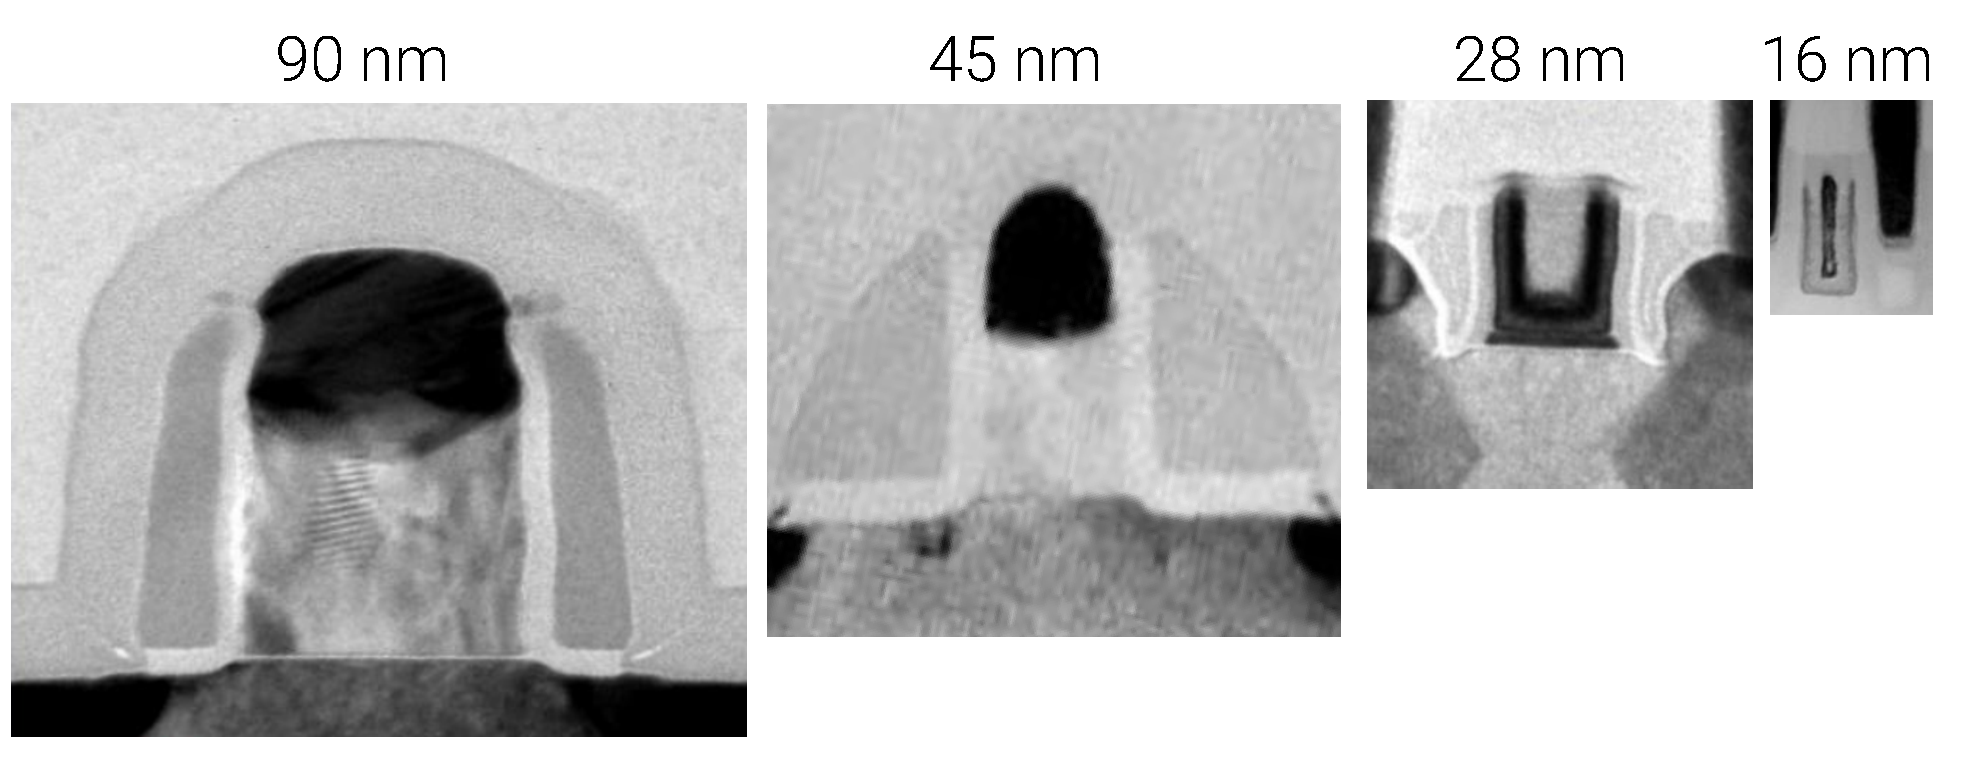
\includegraphics[width=\textwidth]{src/1/figures/technology_evolution.pdf}
  \caption{Recent evolution of NXP's automotive technology nodes \cite{evolution_technologies}}
  \label{fig:nxp-techno-increase}
\end{figure}

% Side effects of size reduction
Cette réduction de taille s'accompagne d'une augmentation de la fragilité et de la sensibilité des circuits intégrés.
Les seuils de tolérances en tension et courant deviennent plus petits, au delà desquels les circuits sont détruits.
La surface de silicium nécessaire à la protection des coeurs de circuits occupe une plus large part de l'aire totale d'un produit  \cite{evolution_technologies}, et donc du coût.

% Another trend in automotive - more electronic functions
De nos jours, de nouvelles fonctionnalités majeures sont aussi en dévelopement dans le domaine automobile.
En particulier, les véhicules autonomes ou l'aide à la conduite font leur apparition sur les routes.
Ces fonctionnalités font en permanence des décisions et prennent des actions critiques sur le véhicule, comme tourner le volant ou enclencher le freinage.
Elles sont implémentées afin d'augmenter la sécurité des usagers d'un véhicule, ce qui résulte en des responsabilités et des contraintes accrues sur les modules électroniques.
La sûreté de fonctionnement des ces modules est donc vitale pour ce type d'application.

% Another trend is reduced power consumptions
L'augmentation de la quantité d'électronique dans un véhicule s'accompagne aussi d'une forte hausse de la consommation électrique.
Au niveau circuit-intégré, les tensions d'alimentations sont réduites très bas, avec communément des seuils d'alimentions de 1V.
Les marges de bruit des cellules digitales sont réduites d'autant, rendant les circuits bien plus sensibles aux perturbations électriques.

% Harsh environment in the automotive field
Par ailleurs, l'environnement automobile est très sévère pour les composants électroniques.
Un moteur en fonctionnement génère de la chaleur et des vibrations.
Durant toute sa vie, un véhicule est exposé à de larges cycles thermiques.
Les contacts électriques, les soudures et les connections vieillissent plus rapidement à cause de cela.
De plus, les systèmes électroniques sont exposés à une large plage de stress électriques.
Quand le moteur est allumé, la tension de batterie chute fortement à cause de l'appel de courant créé par le démarreur.
Cette variation très brutale peut affecter ou endommager les modules.
Il existe également une autre famille de perturbations électriques appellée décharges électrostatiques, et produite par l'environnement du véhicule.

% What is an ESD
Une décharge électrostatique est un transfert de charge soudain entre deux objets de différente charge.
C'est le résultat d'une accumulation de potentiel électrostatique.
La décharge se produit lorsque la différence de potentiel est suffisamment large.
L'amplitude de tels événements peut atteindre couramment plusieurs milliers de volts et des dizaines d'ampères.
Le fabricant de véhicules Renault estimes que les composants électroniques automobiles sont exposés 10000 fois à des décharges pendant leur vie \cite{Renault-esd}.

% Architecture systemes automobiles
L'architecture des systèmes électriques dans un véhicule est également très complexe et rude pour les modules électroniques.
Une voiture est consistutées d'une multitude de modules électroniques interconnectés par des câbles.
C'est un vrai challenge pour garantir la robustesse de cet ensemble contre des perturbations électriques.
La seule connection d'une voiture à une vrai référence électrique se fait par les pneus, ce qui équivaut globalement à une très mauvaise connection à la terre.
Néanmoins, les modules électroniques ont besoin d'une bonne référence pour communiquer entre eux et fonctionner correctement.
Ceci est assuré par la carcasse métallique du véhicule.
En statique et à basse fréquence, cette référence est très bonne car très peu résistive.
Les décharges électrostatiques sont au contraire des évènements avec la majorité du spectre à très haute fréquence, jusqu'à 1 GHz environ.
Dans cette gamme de fréquence, la carcasse métallique ne se comporte plus comme une bonne référence et les cables deviennent largement inductifs.
Ces phénomènes peuvent donc fortement perturber les systèmes électroniques.
De plus, les cables peuvent rayonner et les propagations peuvent se propager par couplage.
Globalement, l'architecture d'un véhicule est complex et sensible par nature aux perturbations.

\begin{figure}[!h]
  \centering
  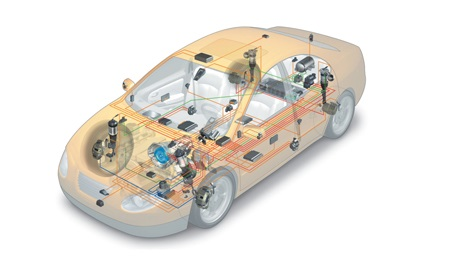
\includegraphics[width=0.7\textwidth]{src/1/figures/systemintegration_01_uv-data.jpg}
  \caption{Architecture of electronic systems in a vehicle \cite{car-architecture}}
  \label{fig:car-architecture}
\end{figure}

% Fiabilite vis a vis des ESD
En résumé, la quantité de composants électroniques est en augmentation et en parallele ils deviennent de plus en plus sensibles.
De plus, ils doivent opérer dans une environnement électrique sévère, avec de multiples sources de perturbation.
Ces perturbations peuvent créer des défaillances.
Dans le domaine des décharges électrostatiques, il y a deux types de défaillances à considérer.
La casse matérielle est le résultat de la destruction permanente d'un composant.
Les circuits intégrés sont particulièrement vulnérables \cite{impactESDsemiconductors} et nécessitent des mesures de protection.
Récemment, un deuxième type de défaillance commence à être étudié.
Les défaillances fonctionnelles sont une perturbation d'une fonction électrique du circuit intégré à la suite d'une décharge.
Plusieurs niveaux de sévérité existent.
La perturbation du système d'airbag est par exemple bien plus critique celle du système de tableau de bord.

\begin{figure}[!h]
  \centering
  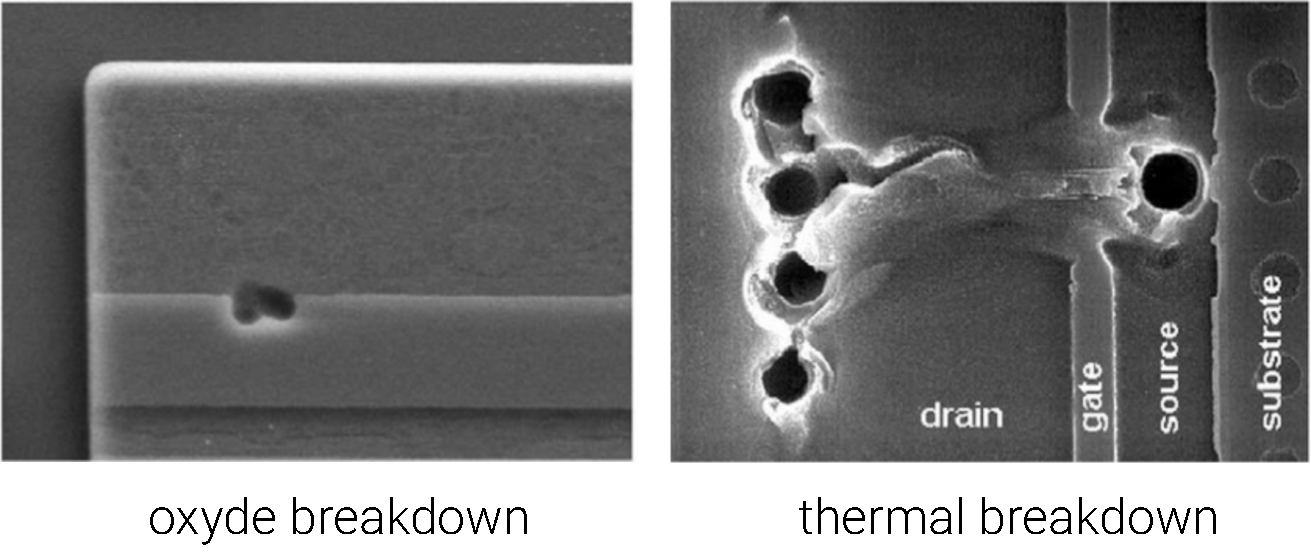
\includegraphics[width=0.4\textwidth]{src/1/figures/esd_failures.jpg}
  \caption{Different kinds of ESD-induced failures}
  \label{fig:esd-failures}
\end{figure}

% Comment predire ces defaillances fonctionnelles
First research on the topic was published by F. Caignet and N. Lacrampe in 2007 \cite{}.
After a few years, the industry widely acknowledged the problem, reinforced by the current automotive trends.
A large amount of research at the system level was published in EOS/ESD symposia 2012 \cite{} and 2013 \cite{}.
The draft standard IEC 62433-6 aims to provide a base framework for soft-failures analysis and prediction.
So far, the litterature is focused on system-level analysis.
There is currently no real work at the component level or studies performed inside the design of an integrated circuit.
This PhD explored the topic and tries to provide some new leads for future research.

% Presentation des chapitres
%
Chapter \ref{chap:1} details how electrostatic discharge physically appear, how to reproduce them in laboratory conditions and summarizes recent litterature.
This preliminary work highlights how functional failures appear and how they impact electronic devices.
It is demonstrated that so far integrated circuits are studied as black-box electrical objects.
Stresses are injected on external inputs while external outputs are monitored for failures.
The amount of silicon-level studies and research remains small.

%
Chapter \ref{chap:2} presents a modeling method for simulating \gls{esd} waveforms up to the integrated circuit inputs.
The first challenge for understanding soft-failures at silicon-level is to determine what fraction of an incoming \gls{esd} actually reaches the integrated circuit.
Between the injection point of a stress and the disturbed circuit, many devices are be connected such as cables, discrete devices, etc.
Each element interacts with the discharge, absorbs a part of its current or changes the waveform.
A model library of common electrical elements found in \gls{esd} testing environment has been constructed and is detailed.

%
A case of soft-failure in an integrated circuit is explained in chapter \ref{chap:3}.
In a first phase, measurement data is obtained at the board level and the failure is explained.
Simulations are run to understand how failures appear, and more specifically how a short electrical event can disturb an integrated circuit for a long period of time.
In a second phase, the integrated function is placed onto a custom testchip.
Specific on-silicon structures were designed to gather measurement data on electrical nets that are not physically accessible.
All these measurements are performed for the purpose of estimating the accuracy of integrated circuit \gls{esd} simulations.
There are two main potential sources of error that are checked.
Silicon technology device models are not designed to function for extremely fast transient transient disturbances.
Also, standard simulations do not take parasitic devices into account, such as metal track resistances and parasitic couplings.
Measurement data is confronted to simulations in order to verify the validity of models.
Analysis of the failure led to the development of a testchip, to put on silicon the same failing function but with a more convenient environment for measurements and investigation.

%
When issues are discovered late in the testing lab, analysis is performed manually, by trial and error, searching inside the design why the function is failing.
It is a complex and time-consuming process.
The core research of this work focuses proposing new analysis methods and tools for electrical simulations.
It is detailled in chapter \ref{sec:methods-operating-esd-analysis}.

%
Finally, a new test generator was developed to overcome some issues found when debugging silicon-level failures caused by system level \gls{esd} testers.
The principle of operation and architecture of the generator is described in chapter \ref{sec:tlp-hmm}.
The conclusion summarizes the work achieved during the PhD, highlights the most notable discoveries, and identifies follow-up work and research topics that could be worth pursuing.
Some part of the research work also focused towards \gls{esd} testers.
System-level \gls{esd} guns \cite{iec61000-4-2, iso10605} constitute a major testing and qualification tool, but bring too much complexity during silicon-level investigation.
To overcome this issue, a new stress generator based on a \gls{tlp} is proposed in chapter \ref{sec:tlp-hmm}.
It produces the same compliant waveform than those standards, but with some interesting advantages.
It is not a drop-in replacement but can be interesting as an investigation tool.

%
Final conclusions and potential following work are detailed in chapter \ref{sec:final-conclusion}.
